%&preformat-disser
\RequirePackage[l2tabu,orthodox]{nag} % Раскомментировав, можно в логе получать рекомендации относительно правильного использования пакетов и предупреждения об устаревших и нерекомендуемых пакетах
% Формат А4, 14pt (ГОСТ Р 7.0.11-2011, 5.3.6)
\documentclass[a4paper,14pt,oneside,openany]{memoir}

%%%%%%%%%%%%%%%%%%%%%%%%%%%%%%%%%%%%%%%%%%%%%%%%%%%%%%%%%%%%%%%%%%%%%%%%%%%%%%%%
%%%% Файл упрощённых настроек шаблона, общих для диссертации и автореферата %%%%
%%%%%%%%%%%%%%%%%%%%%%%%%%%%%%%%%%%%%%%%%%%%%%%%%%%%%%%%%%%%%%%%%%%%%%%%%%%%%%%%

%%% Режим черновика %%%
\makeatletter
\@ifundefined{c@draft}{
  \newcounter{draft}
  \setcounter{draft}{1}  % 0 --- чистовик (максимальное соблюдение ГОСТ)
                         % 1 --- черновик (отклонения от ГОСТ, но быстрая
                         %       сборка итоговых PDF)
}{}
\makeatother

%%% Пометки в тексте %%%
\makeatletter
\@ifundefined{c@showmarkup}{
  \newcounter{showmarkup}
  \setcounter{showmarkup}{0}  % 0 --- скрыть пометки
                              % 1 --- показывать пометки
}{}
\makeatother

%%% Использование в pdflatex шрифтов не по-умолчанию %%%
\makeatletter
\@ifundefined{c@usealtfont}{
  \newcounter{usealtfont}
  \setcounter{usealtfont}{1}    % 0 --- шрифты на базе Computer Modern
                                % 1 --- использовать пакет pscyr, при его
                                %       наличии
                                % 2 --- использовать пакет XCharter, при наличии
                                %       подходящей версии
}{}
\makeatother

%%% Использование в xelatex и lualatex семейств шрифтов %%%
\makeatletter
\@ifundefined{c@fontfamily}{
  \newcounter{fontfamily}
  \setcounter{fontfamily}{1}  % 0 --- CMU семейство. Используется как fallback;
                              % 1 --- Шрифты от MS (Times New Roman и компания)
                              % 2 --- Семейство Liberation
}{}
\makeatother

%%% Библиография %%%
\makeatletter
\@ifundefined{c@bibliosel}{
  \newcounter{bibliosel}
  \setcounter{bibliosel}{1}   % 0 --- встроенная реализация с загрузкой файла
                              %       через движок bibtex8;
                              % 1 --- реализация пакетом biblatex через движок
                              %       biber
}{}
\makeatother

%%% Предкомпиляция tikz рисунков для ускорения работы %%%
\makeatletter
\@ifundefined{c@imgprecompile}{
  \newcounter{imgprecompile}
  \setcounter{imgprecompile}{1}   % 0 --- без предкомпиляции;
                                  % 1 --- пользоваться предварительно
                                  %       скомпилированными pdf вместо генерации
                                  %       заново из tikz
}{}
\makeatother
            % общие настройки шаблона
\input{common/packages}         % Пакеты общие для диссертации и автореферата
\synopsisfalse                      % Этот документ --- не автореферат
\input{Dissertation/dispackages}    % Пакеты для диссертации
\usepackage{fr-longtable}    %ради \endlasthead

% Листинги с исходным кодом программ
\usepackage{fancyvrb}
\usepackage{listings}
\lccode`\~=0\relax %Без этого хака из-за особенностей пакета listings перестают работать конструкции с \MakeLowercase и т. п. в (xe|lua)latex

% Русская традиция начертания греческих букв
\usepackage{upgreek} % прямые греческие ради русской традиции

%%% Микротипографика
%\ifnumequal{\value{draft}}{0}{% Только если у нас режим чистовика
%    \usepackage[final, babel, shrink=45]{microtype}[2016/05/14] % улучшает представление букв и слов в строках, может помочь при наличии отдельно висящих слов
%}{}

% Отметка о версии черновика на каждой странице
% Чтобы работало надо в своей локальной копии по инструкции
% https://www.ctan.org/pkg/gitinfo2 создать небходимые файлы в папке
% ./git/hooks
% If you’re familiar with tweaking git, you can probably work it out for
% yourself. If not, I suggest you follow these steps:
% 1. First, you need a git repository and working tree. For this example,
% let’s suppose that the root of the working tree is in ~/compsci
% 2. Copy the file post-xxx-sample.txt (which is in the same folder of
% your TEX distribution as this pdf) into the git hooks directory in your
% working copy. In our example case, you should end up with a file called
% ~/compsci/.git/hooks/post-checkout
% 3. If you’re using a unix-like system, don’t forget to make the file executable.
% Just how you do this is outside the scope of this manual, but one
% possible way is with commands such as this:
% chmod g+x post-checkout.
% 4. Test your setup with “git checkout master” (or another suitable branch
% name). This should generate copies of gitHeadInfo.gin in the directories
% you intended.
% 5. Now make two more copies of this file in the same directory (hooks),
% calling them post-commit and post-merge, and you’re done. As before,
% users of unix-like systems should ensure these files are marked as
% executable.
\ifnumequal{\value{draft}}{1}{% Черновик
   \IfFileExists{.git/gitHeadInfo.gin}{
      \usepackage[mark,pcount]{gitinfo2}
      \renewcommand{\gitMark}{rev.\gitAbbrevHash\quad\gitCommitterEmail\quad\gitAuthorIsoDate}
      \renewcommand{\gitMarkFormat}{\rmfamily\color{Gray}\small\bfseries}
   }{}
}{}
\usepackage[version=4]{mhchem} %Chemistry
   % Пакеты для специфических пользовательских задач

%%%%%%%%%%%%%%%%%%%%%%%%%%%%%%%%%%%%%%%%%%%%%%%%%%%%%%%%%%%%%%%%%%%%%%%%%%%%%%%%
%%%% Файл упрощённых настроек шаблона, общих для диссертации и автореферата %%%%
%%%%%%%%%%%%%%%%%%%%%%%%%%%%%%%%%%%%%%%%%%%%%%%%%%%%%%%%%%%%%%%%%%%%%%%%%%%%%%%%

%%% Режим черновика %%%
\makeatletter
\@ifundefined{c@draft}{
  \newcounter{draft}
  \setcounter{draft}{1}  % 0 --- чистовик (максимальное соблюдение ГОСТ)
                         % 1 --- черновик (отклонения от ГОСТ, но быстрая
                         %       сборка итоговых PDF)
}{}
\makeatother

%%% Пометки в тексте %%%
\makeatletter
\@ifundefined{c@showmarkup}{
  \newcounter{showmarkup}
  \setcounter{showmarkup}{0}  % 0 --- скрыть пометки
                              % 1 --- показывать пометки
}{}
\makeatother

%%% Использование в pdflatex шрифтов не по-умолчанию %%%
\makeatletter
\@ifundefined{c@usealtfont}{
  \newcounter{usealtfont}
  \setcounter{usealtfont}{1}    % 0 --- шрифты на базе Computer Modern
                                % 1 --- использовать пакет pscyr, при его
                                %       наличии
                                % 2 --- использовать пакет XCharter, при наличии
                                %       подходящей версии
}{}
\makeatother

%%% Использование в xelatex и lualatex семейств шрифтов %%%
\makeatletter
\@ifundefined{c@fontfamily}{
  \newcounter{fontfamily}
  \setcounter{fontfamily}{1}  % 0 --- CMU семейство. Используется как fallback;
                              % 1 --- Шрифты от MS (Times New Roman и компания)
                              % 2 --- Семейство Liberation
}{}
\makeatother

%%% Библиография %%%
\makeatletter
\@ifundefined{c@bibliosel}{
  \newcounter{bibliosel}
  \setcounter{bibliosel}{1}   % 0 --- встроенная реализация с загрузкой файла
                              %       через движок bibtex8;
                              % 1 --- реализация пакетом biblatex через движок
                              %       biber
}{}
\makeatother

%%% Предкомпиляция tikz рисунков для ускорения работы %%%
\makeatletter
\@ifundefined{c@imgprecompile}{
  \newcounter{imgprecompile}
  \setcounter{imgprecompile}{1}   % 0 --- без предкомпиляции;
                                  % 1 --- пользоваться предварительно
                                  %       скомпилированными pdf вместо генерации
                                  %       заново из tikz
}{}
\makeatother
      % Упрощённые настройки шаблона

% Новые переменные, которые могут использоваться во всём проекте
% ГОСТ 7.0.11-2011
% 9.2 Оформление текста автореферата диссертации
% 9.2.1 Общая характеристика работы включает в себя следующие основные структурные
% элементы:
% актуальность темы исследования;
\newcommand{\actualityTXT}{Актуальность темы.}
% степень ее разработанности;
\newcommand{\progressTXT}{Степень разработанности темы.}
% цели и задачи;
\newcommand{\aimTXT}{Целью}
\newcommand{\tasksTXT}{задачи}
% научную новизну;
\newcommand{\noveltyTXT}{Научная новизна:}
% теоретическую и практическую значимость работы;
%\newcommand{\influenceTXT}{Теоретическая и практическая значимость}
% или чаще используют просто
\newcommand{\influenceTXT}{Практическая значимость}
% методологию и методы исследования;
\newcommand{\methodsTXT}{Методология и методы исследования.}
% положения, выносимые на защиту;
\newcommand{\defpositionsTXT}{Основные положения, выносимые на~защиту:}
% степень достоверности и апробацию результатов.
\newcommand{\reliabilityTXT}{Достоверность}
\newcommand{\probationTXT}{Апробация работы.}

\newcommand{\contributionTXT}{Личный вклад.}
\newcommand{\publicationsTXT}{Публикации.}


%%% Заголовки библиографии:

% для автореферата:
\newcommand{\bibtitleauthor}{Публикации автора по теме диссертации}

% для стиля библиографии `\insertbiblioauthorgrouped`
\newcommand{\bibtitleauthorvak}{В изданиях из списка ВАК РФ}
\newcommand{\bibtitleauthorscopus}{В изданиях, входящих в международную базу цитирования Scopus}
\newcommand{\bibtitleauthorwos}{В изданиях, входящих в международную базу цитирования Web of Science}
\newcommand{\bibtitleauthorother}{В прочих изданиях}
\newcommand{\bibtitleauthorconf}{В сборниках трудов конференций}

% для стиля библиографии `\insertbiblioauthorimportant`:
\newcommand{\bibtitleauthorimportant}{Наиболее значимые \protect\MakeLowercase\bibtitleauthor}

% для списка литературы в диссертации и списка чужих работ в автореферате:
\newcommand{\bibtitlefull}{Список литературы} % (ГОСТ Р 7.0.11-2011, 4)
%\newcommand\reaction[1][2]{\begin{equation}\ce{#1} \label[2] \end{equation}}

%\newcommand\reactionnonumber[1]%
%    {\begin{equation*}\ce{#1}\end{equation*}}
%
%\newcommand\reaction@[2][]%
%    {\begin{equation}\ce{#2}%
%    \ifx\@empty#1\@empty\else\label{#1}\fi%
%    \reactiontag\end{equation}}

\makeatletter
\newcounter{reaction}
%%% >> for article <<%
\renewcommand\thereaction{Х.\,\arabic{reaction}}
%%% << for article <<
%%%>> for report and book >>
\renewcommand\thereaction{Х.\,\thechapter.\arabic{reaction}}
\@addtoreset{reaction}{chapter}
%%% << for report and book <<
\newcommand\reactiontag%
    {\refstepcounter{reaction}\tag{\thereaction}}
\newcommand\reaction@[2][]%
    {\begin{equation}\ce{#2}%
    \ifx\@empty#1\@empty\else\label{#1}\fi%
    \reactiontag\end{equation}}
\newcommand\reaction@nonumber[1]%
    {\begin{equation*}\ce{#1}\end{equation*}}
\newcommand\reaction%
    {\@ifstar{\reaction@nonumber}{\reaction@}}
    \makeatother
         % Новые переменные, для всего проекта

\input{common/data}             % Основные сведения
\input{common/fonts}            % Определение шрифтов (частичное)
\input{common/styles}           % Стили общие для диссертации и автореферата
\input{Dissertation/disstyles}  % Стили для диссертации
\input{Dissertation/userstyles} % Стили для специфических пользовательских задач

%%% Библиография. Выбор движка для реализации %%%
% Здесь только проверка установленного ключа. Сама настройка выбора движка
% размещена в common/setup.tex
\ifnumequal{\value{bibliosel}}{0}{%
    \input{biblio/predefined}   % Встроенная реализация с загрузкой файла через движок bibtex8
}{
    \input{biblio/biblatex}     % Реализация пакетом biblatex через движок biber
}

% Вывести информацию о выбранных опциях в лог сборки
\typeout{Selected options:}
\typeout{Draft mode: \arabic{draft}}
\typeout{Font: \arabic{fontfamily}}
\typeout{AltFont: \arabic{usealtfont}}
\typeout{Bibliography backend: \arabic{bibliosel}}
\typeout{Precompile images: \arabic{imgprecompile}}
% Вывести информацию о версиях используемых библиотек в лог сборки
\listfiles

%%% Управление компиляцией отдельных частей диссертации %%%
% Необходимо сначала иметь полностью скомпилированный документ, чтобы все
% промежуточные файлы были в наличии
% Затем, для вывода отдельных частей можно воспользоваться командой \includeonly
% Ниже примеры использования команды:
%
%\includeonly{Dissertation/part2}
%\includeonly{Dissertation/contents,Dissertation/appendix,Dissertation/conclusion}
%
% Если все команды закомментированы, то документ будет выведен в PDF файл полностью

\begin{document}

\input{common/renames}                 % Переопределение именований

%%% Структура диссертации (ГОСТ Р 7.0.11-2011, 4)
\include{Dissertation/title}           % Титульный лист
\include{Dissertation/contents}        % Оглавление
\ifnumequal{\value{contnumfig}}{1}{}{\counterwithout{figure}{chapter}}
\ifnumequal{\value{contnumtab}}{1}{}{\counterwithout{table}{chapter}}
%\include{Dissertation/introduction}    % Введение
\ifnumequal{\value{contnumfig}}{1}{\counterwithout{figure}{chapter}
}{\counterwithin{figure}{chapter}}
\ifnumequal{\value{contnumtab}}{1}{\counterwithout{table}{chapter}
}{\counterwithin{table}{chapter}}
\chapter{Литературный обзор}%
\label{cha:Литературный обзор}
\section{Гексагональный нитрид бора}%
\label{sec:Гексагональный нитрид бора}

Гексагональный нитрида бора (h-BN) по своей структуре аналог графита, поэтому
иногда называют "белым графитом". Кристаллическая структура h-BN представляет
из себя набор графеноподобных слоев, расположенных, в отличие от структуры 
графита точно один под другим с чередованием атомов B и N по оси Z. Расстояние 
между слоями в решетке нитрида бора равно 3,34 А, которое меньше, чем у графита
(3,40 А), что доказывает о более прочной связи между слоями в структуре BN.

Температура плавления h-BN под давлением азота больше 3000 °С, плотность 
составляет \SI{2.3}{\gram\per\cm^3} Гексагональный BN обладает полупроводниковыми свойствами
(с шириной запрещенной зоны около 3,7 эВ), так же обладает люминесцентными 
свойствами при наличии небольшого количества примесей. Нитрид бора при 
комнатной температуре химически инертен, он практически не реагирует с 
кислородом или хлором, кислотами или щелочами. Подвергается действию кислорода 
и хлора при температурах выше 700 °С. Вступает в реакцию с фтором (образуя \ce{BF3} 
и \ce{N2}) и с HF (образуя \ce{NH4BF4}); горячие растворы щелочей разлагают его с 
выделением \ce{NH3}.

Нитрид бора обладает превосходными антифрикционными свойствами. Нанопорошки
а так же покрытия нитрида бора широко используются в качестве сухой смазки [].
Данная особенность связана с сильной ковалентной связью между B - N базовой плоскости 
связанных между собой слабой Ван-дер-Ваальсой связью [].

\subsection{Методы получения гексагонального нитрида бора}%
\label{sub:Методы получения гексагонального нитрида бора}


Широко распространены следующие методы синтеза гексагонального нитрида бора:

\begin{itemize}
    \item Плазмотермический
    \item Метод СВС
    \item Методы химического осаждения
    \item Методы прямого синтеза
\end{itemize}

В самом общем случае синтез нитрида бора происходит по простой реакции \ce{B + N2}, 
которая может быть осуществлена в трубчатой печи сопротивления. Однако энергия, которую 
необходимо затратить на активацию молекулы \ce{Na} достаточно высока [конкретное
значение], а технологические требования к морфологии и структуре материала ставят
задачи по поиску новых, оптимальных методик по синтезу различных структур. 

\subsection{Газовое восстановление}%
\label{sub:Газовое востановление}

Первые исследовательские работы по изучению синтеза гексагонального BN учитывали
необходимость замены реагентов на прекурсоры с  меньшей энергией активации для 
прохождения реакции. Одним из решений может являться
замена \ce{N2} на \ce{NH4}, а чистого аморфного бора на \ce{H3BO3}. Первые
работы в области синтеза BN структур показали образование различных переходных 
продуктов: \ce{(B2O3)nNH} при \SI{200}{\degreeCelsius},
\ce{(BN)x(B2O3)y(NH3)z} при \SI{350}{\degreeCelsius}
\cite[]{economy_boron_1967}. Образование оксида бора с точкой плавления
\SI{450}{\degreeCelsius} приводит уменьшению удельной поверхности при
температурах выше температуры плавления, что приводит к агломерации
капель оксида бора и уменьшению контактной поверхности между реакционным
газом и прекурсором. Подобный эффект негативно сказывается на диффузии реакционного
газа через прекурсор, в результате чего в продуктах реакции наблюдается большое 
количество непрореагировавших реагентов, а так же полупродуктов. Чтобы преодолеть
данное технологическое ограничение синтез проводился в несколько этапов: синтез
в протоке реакционного газа прерывался, полупродукт перемалывался, далее синтез
возобновляли. Так же существенным технологическим осложнением являлось 
использование аммиака в качестве источника атомарного азота.

Для решения данной проблемы обычно используют инертные наполнители или
продукты реакции, которые не реагируют с исходными компонентами и газовой
средой, а так же не дают мельчайшим каплям оксида бора сливаться. И тут
возникает некоторая дилемма. С одной стороны, использование в качестве
наполнителя продукта реакции должно увеличивать чистоту выходящих
продуктов. Однако, в одной из первых работ, было показано что
использование альтернативных наполнителей (например ортофосфата кальция)
значительно увеличивает долю выхода BN в отношении к полупродуктам
\cite[]{basu_synthesis_1990}. С другой, использование альтернативных
наполнителей приводит к появлению дополнительных операций очистки BN от
примесей. Так же оставалась проблема синтеза частиц BN контролируемой
размерности и морфологии. Если с размерностью можно было справится
постобработкой готовых порошков (размол в шаровой мельнице [ссылка]
и др.), то синтез новых структурных модификаций требовал пересмотра
традиционного подхода.

Одним из первых промышленных процессов синтеза гексагонального нитрида бора является
процесс О'Конора \cite[]{edmond_process_1966}. Данный метод основан на взаимодействии 
борной кислоты и карбамида:

\reaction{(NH2)2CO + 2H3BO3 -> 2BN + CO2 + 5H2O}

Исходную смесь карбамида и нитрида бора спекают при температуре 
\SIrange{200}{300}{\degreeCelsius}, далее спек измельчают термообрабатывают в протоке 
азота и аммиака при температуре \SIrange{800}{1200}{\degreeCelsius}. Данный метод
широко применяется в синтезе микро- и нанопорошков \ce{h-BN}. Основным недостатком
данного метода является высокая турбостратность структуры целевого продукта.
Использование данного метода не позволяет получить материал контролируемой 
графитоподобной структуры, а так же материал, полученный данным методом 
обладает высоким индексом графитации ("g" > 4).  


В 2005 году был зарегистрирован патент \cite[]{_ru__2005} развивающий данный 
подход к синтезу гексагонального нитрида бора. Группа исследователей под
руководством А.~С.~Нечепуренко разработали метод синтеза гексагонального нитрид
бора, позволяющий получить материал однородной структуры с контролируемо-низким
индексом графитации ("g" \ge 1.7). Ключевой особенностью прилагаемого метода
является предварительное деление исходной шихты \ce{(NH2)2CO + 2H3BO3} на две части 
различных по соотношению карбамида к борной кислоте, а так же их предварительной
термической обработки до \SI{400}{\degreeCelsius}. При температуре \SI{400}{\degreeCelsius}
спеки смешивают и размалывают в соотношении, которое соответствует необходимому 
индексу графитации конечного продукта, после чего спек азотируют в среде \ce{N2}
при температуре \SI{1850}{\degreeCelsius}.

Полученный нитрид бора имеет чистоту \SI{98.8}{\text{масс.}\%} и примесью по 
борному ангидриту около \SI{0.12}{\text{масс.}\%}.

\subsection{Метод самораспространяющегося высокотемпературного синтеза}%
\label{sub:Метод самораспространяющегося высокотемпературного синтеза}

Большим прорывом в синтезе нитридных керамик стало открытие процессов
самораспространяющегося высокотемпературного синтеза (СВС). Ведущую роль
в открытии и развитии методов СВС сыграла группа советских
исследователей: И.~П.~Боровинская, В.~М.~Ширко и А.~Г.~Мержанов. Достижения
в области СВС позволили пересмотреть промышленный подход к синтезу нитрида
бора. Ключевой особенность СВС является синтез конечного продукта благодаря
энергии выделяющейся в ходе экзотермической реакции. Использование методов 
СВС для синтеза нитридных керамик привело к существенной экономии на затрачиваемой
энергии.

Графитоподобный нитрид бора можно получить горением аморфного бора под давлением 
азота с большим выделением энергии \cite[]{loryan_nanosized_2009}:

\reaction[che:shs_BN]{2B + N2 -> 2BN + Q}

Из аморфного бора прессуют объемную заготовку \SI{0.21}{\gram\per\cm^3} в среде
азота. Далее под давлением \SIrange{10}{150}{\mega\pascal} совершается
инициирование реакции. При увеличении давления \ce{N2}  уменьшается количество
исходного аморфного бора в продуктах реакции вплоть до 0.1 масс.\% при давлении 
\SI{100}{\mega\pascal}. Температура горения достигала \SIrange{2473}{2523}{\kelvin}

Однако, данный способ имеет значимое технологическое ограничение: требование 
по наличию азотной атмосферы под столь высоким давлением может привести к значительным сложностям
с точки зрения промышленной безопасности и технологичности производства.

Альтернативный способ синтеза порошка гексагонального нитрида бора был запатентован 
группой И.~П.~Боровинской в 1999~в. \cite[]{__1999}.

Данный патент основывается на методе восстановления оксида бора в присутствии магния
в атмосфере азота:

\reaction[chem:bn_shs_mg]{B2O3 + 3Mg + N2 -> 2BN + 3MgO + Q}

Синтез готового порошка проводится в несколько этапов: подготовка реакционной смеси,
запресовка, инициирование реакции, забор и размол продуктов реакции, чистка от примесей,
сушка. Давление азота в камере составляет \SIrange{8}{10}{\mega\pascal}. Очистка 
целевого продукта проводится путем обработки продуктов синтеза 
\SIrange{10}{26}{\%}-серной кислотой.  

Рекомендуемое соотношение реагентов: \ce{B2O3}~48~масс.\%, \ce{Mg}~32~масс.\%., 
а так же смесь реагентов в соотношении 30~масс.\%~\ce{\text{h-}BN} и 
70~масс.\%~\ce{MgO}. Так же, продуктами реакции покрывается графитовая подложка
реактора, а так же боковые стенки. Реакция протекает в течение 7 минут и при
температуре \SI{1800}{\degreeCelsius}.  

Продукты реакции добавляются в исходную смесь с целью уменьшения скорости реакции, 
а также уменьшения температуры горения. В сравнении с методом~\ref{che:shs_BN} 
реакция протекает при значительно более низких температурах. Благодаря более низкой
температуре в продуктах реакции отсутствуют следы плавления \ce{BN}, а так же 
исключает образование сложноудаляемых боридов магния. После отмывки продуктов
в \SI{20}{\%}-ной серной кислоте при температуре \SI{100}{\degreeCelsius}
и последующей промывки водой целевой продукт содержит гексагональный нитрид бора.
Выход готовой продукции составляет \SI{22}{\%}, что соответствует \SI{98}{\%}  
относительно исходного \ce{B2O3}. 

Как можно увидеть, способ получения графитоподобного нитрида бора,
запатентованный Боровинской \cite[]{__1999}, отличается большей технологичностью
и экономичностью в связи меньшими затратами \ce{N2}, а так же отсутствию необходимости
постоянного перемешивания и размола полупродуктов.

Другим распространенным методом получения является азидная технология СВС.

%\begin{figure}[ht]
%    \centering
%    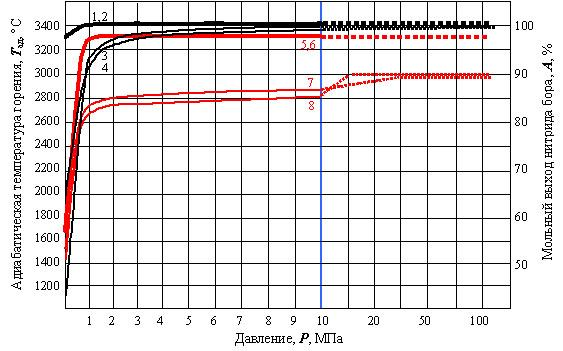
\includegraphics[width=0.8\textwidth]{BN-SHS.png}
%    \caption{Зависимость адиабатической температуры горения систем~СВС}
%\legend{1,2 – мольный выход BN в системе \ce{4B-3NaN3-NH4Cl}(\ce{NH4Cl}) \\
%        3 – мольный выход BN в системе \ce{8B-3NaN3–KB4} \\
%        4 – мольный выход BN в системе \ce{12B-4NaN3–NH4BF4} \\
%        5 – адиабатическая температура горения в системе \ce{12B - 4NaN3 – NH4BF4} \\
%        6 – адиабатическая температура горения в системе \ce{8B - 3NaN3 – KBF4} \\ 
%       7 – адиабатическая температура горения в системе \ce{4B - NaN3 - NH4Cl}\\
%       8 – адиабатическая температура горения в системе \ce{4B - NaN3 - NH4F}\\
%        }
%    \label{fig:BN-SHS}
%\end{figure}


\begin{figure}[ht]
    \centerfloat{
    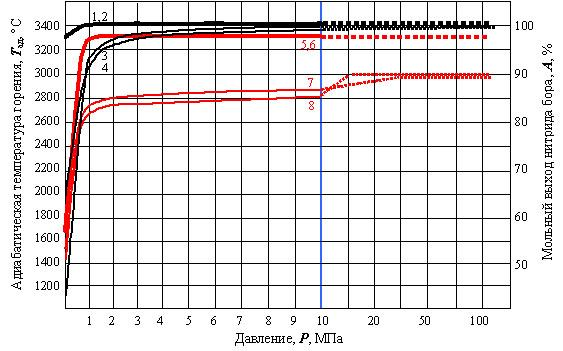
\includegraphics[scale=0.85]{BN-SHS}
    }
    \legend{1,2 – мольный выход BN в системе \ce{4B} - \ce{3NaN3} - \ce{NH4Cl} \\
    3 – мольный выход BN в системе \ce{8B} - \ce{3NaN3} – \ce{KB4} \\ 
    4 – мольный выход BN в системе \ce{12B} - \ce{4NaN3} – \ce{NH4BF4} \\
    5 – адиабатическая температура горения в системе \ce{12B} - \ce{4NaN3} – \ce{NH4BF4} \\
    6 – адиабатическая температура горения в системе \ce{8B} - \ce{3NaN3} – \ce{KBF4} \\ 
    7 – адиабатическая температура горения в системе \ce{4B} - \ce{3NaN3} - \ce{NH4Cl} \\
    8 – адиабатическая температура горения в системе \ce{4B} - \ce{NaN3} - \ce{NH4F} \\
    }
    \caption{Зависимость адиабатической температуры горения систем~СВС}\label{fig:BN-SHS}
\end{figure}

\reaction{4B + NaN_3 + Na4Cl -> 4 BN + NaCl + 2H_2}
\reaction{4B + NaN_3 + NH_4F -> 4 BN + NaF + 2H_2}
\reaction{4B + 3NaN_3 + KBF_4 -> 9 BN + 3NaF + KF}
\reaction{12B + 4NaNa_2 + NH_4BF_4 -> 13 BN + NaCl + 2H_2}

\section{Основные виды наноструктур гексагонального нитрида бора}%
\label{sec:Основные виды наноструктур гексагонального нитрида бора}

 

\begin{itemize}
    \item Сферы 
    \item Нанотрубки
    \item Нанолисты
    \item Игольчатые структуры
\end{itemize}

\subsection{Наносферы}%
\label{sub:Наносферы}


\subsection{Нанотрубки}%
\label{sub:Нанотрубки}


Данная структурная модификация BN нашла широкое применение в самых 
различных областях 

\subsection{Нанолисты}%
\label{sub:Нанолисты}

\subsection{Наноиглы}%
\label{sub:Наноиглы}




%\include{Dissertation/part1}           % Глава 1
%\include{Dissertation/part2}           % Глава 2
%\include{Dissertation/part3}           % Глава 3
%\include{Dissertation/conclusion}      % Заключение
%\include{Dissertation/acronyms}        % Список сокращений и условных обозначений
%\include{Dissertation/dictionary}      % Словарь терминов
\include{Dissertation/references}      % Список литературы
\include{Dissertation/lists}           % Списки таблиц и изображений (иллюстративный материал)

%%% Настройки для приложений
\appendix
% Оформление заголовков приложений ближе к ГОСТ:
\setlength{\midchapskip}{20pt}
\renewcommand*{\afterchapternum}{\par\nobreak\vskip \midchapskip}
\renewcommand\thechapter{\Asbuk{chapter}} % Чтобы приложения русскими буквами нумеровались

%\include{Dissertation/appendix}        % Приложения

\end{document}
